%!TEX root = ../thesis.tex
This section will go though the process and implementation of our prototype.
\todo{As one of the goals of this prototype has been to implement advanced interaction possibilities into a textile surface without the use of advanced machinery ... something something}
To give an insight into the prototype process as well as the final prototype, we have chosen to split the implementation into three overall iteration steps.
Our hope is that this will give a better understanding of the rationale behind our construction decisions as well as ... something something 

\todo{iteration 1 is longer because we describes the basics osv. ??}

\subsection{Iteration 1}
The goal of our first iteration of the prototype was to ensure that the we had construction principles and the right materials for constructing a touch and pressure sensitive fabric, with only off-the-shelf materials and tools.

For our first simple prototype we applied this principle, inspired by Pressure Sensor Matrix\footnote{http://www.instructables.com/id/Pressure-Sensor-Matrix/}, to construct a 2x3 touch pad in neoprene, seen in figure~\ref{prototype_1}, and a bend sensor for simple testing, also seen in figure~\ref{prototype_1}.
The prototype consists of three layers as depicted in figure~\todo{ref}, connected to an Arduino\footnote{http://www.arduino.cc/} for input/output data that is sent to Processing\footnote{http://processing.org/} for data visualization and to Java for data manipulation.

\begin{figure}[h]
\centering
\begin{subfigure}{.5\textwidth}
  \centering
  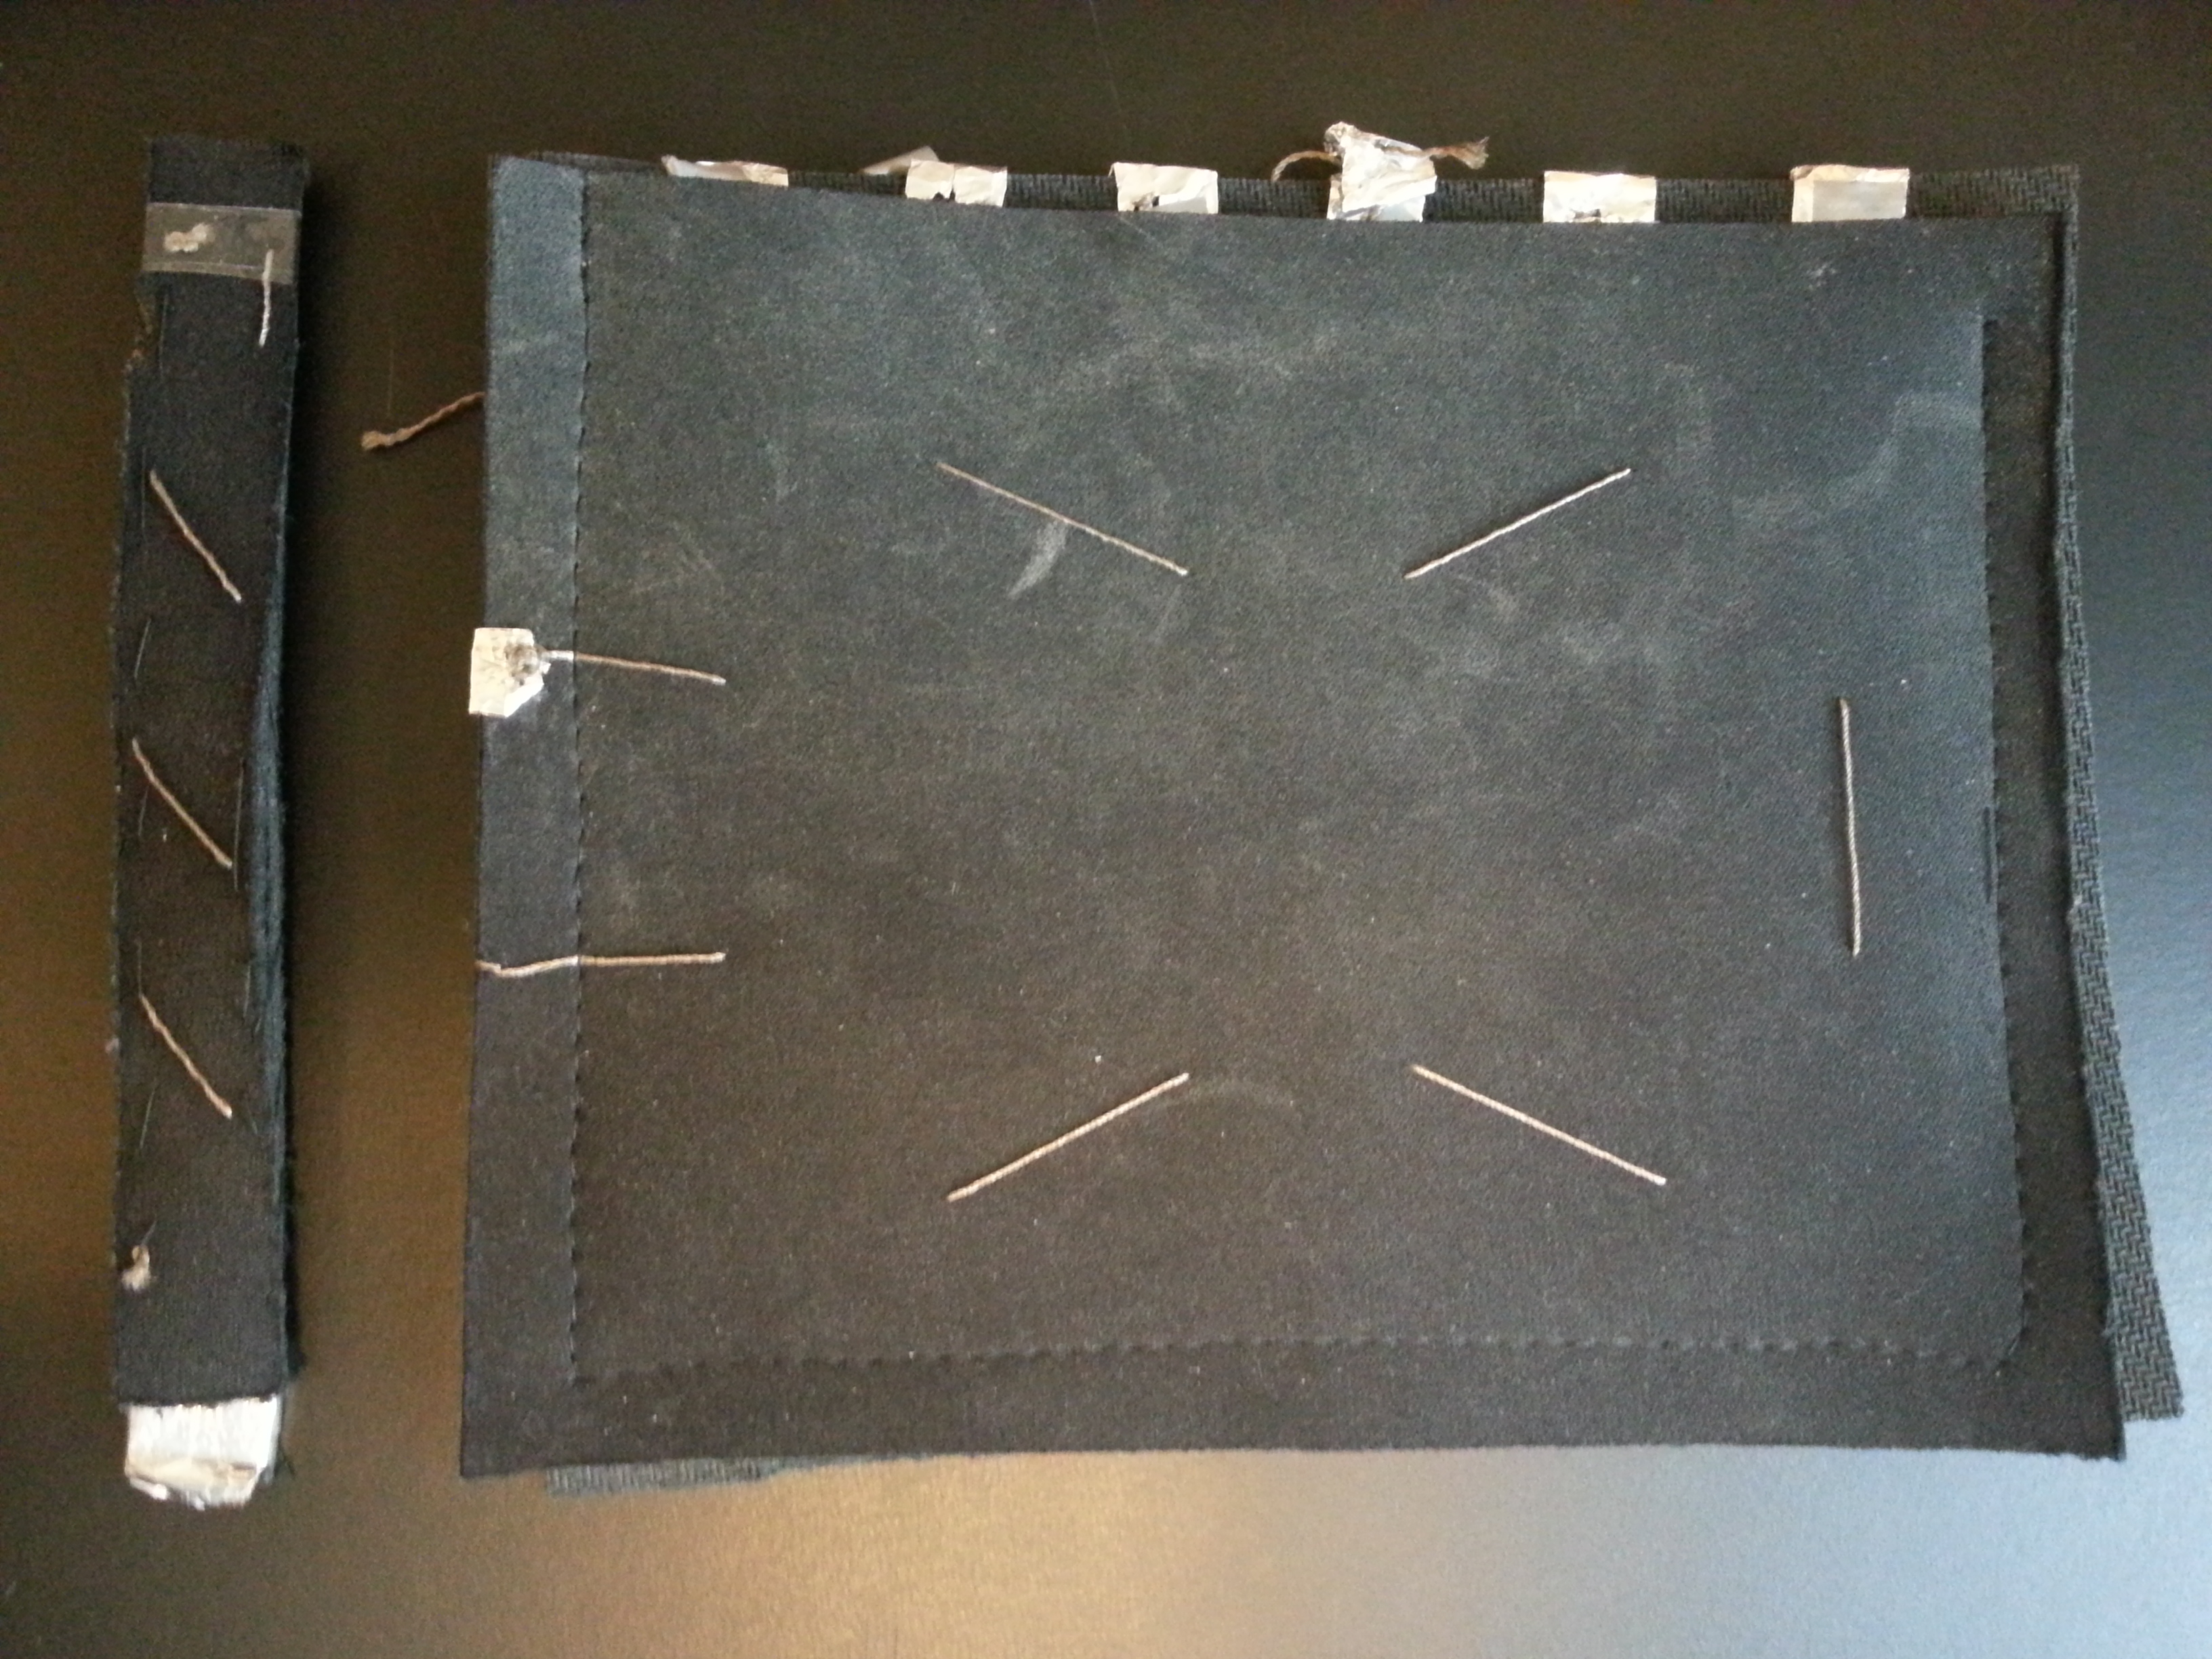
\includegraphics[width=.9\linewidth]{figures/touch/proto1_1}
  \caption{On the left is our simple bend sensor and on the right our 2x3 pressure matrix}
\end{subfigure}%
\begin{subfigure}{.5\textwidth}
  \centering
  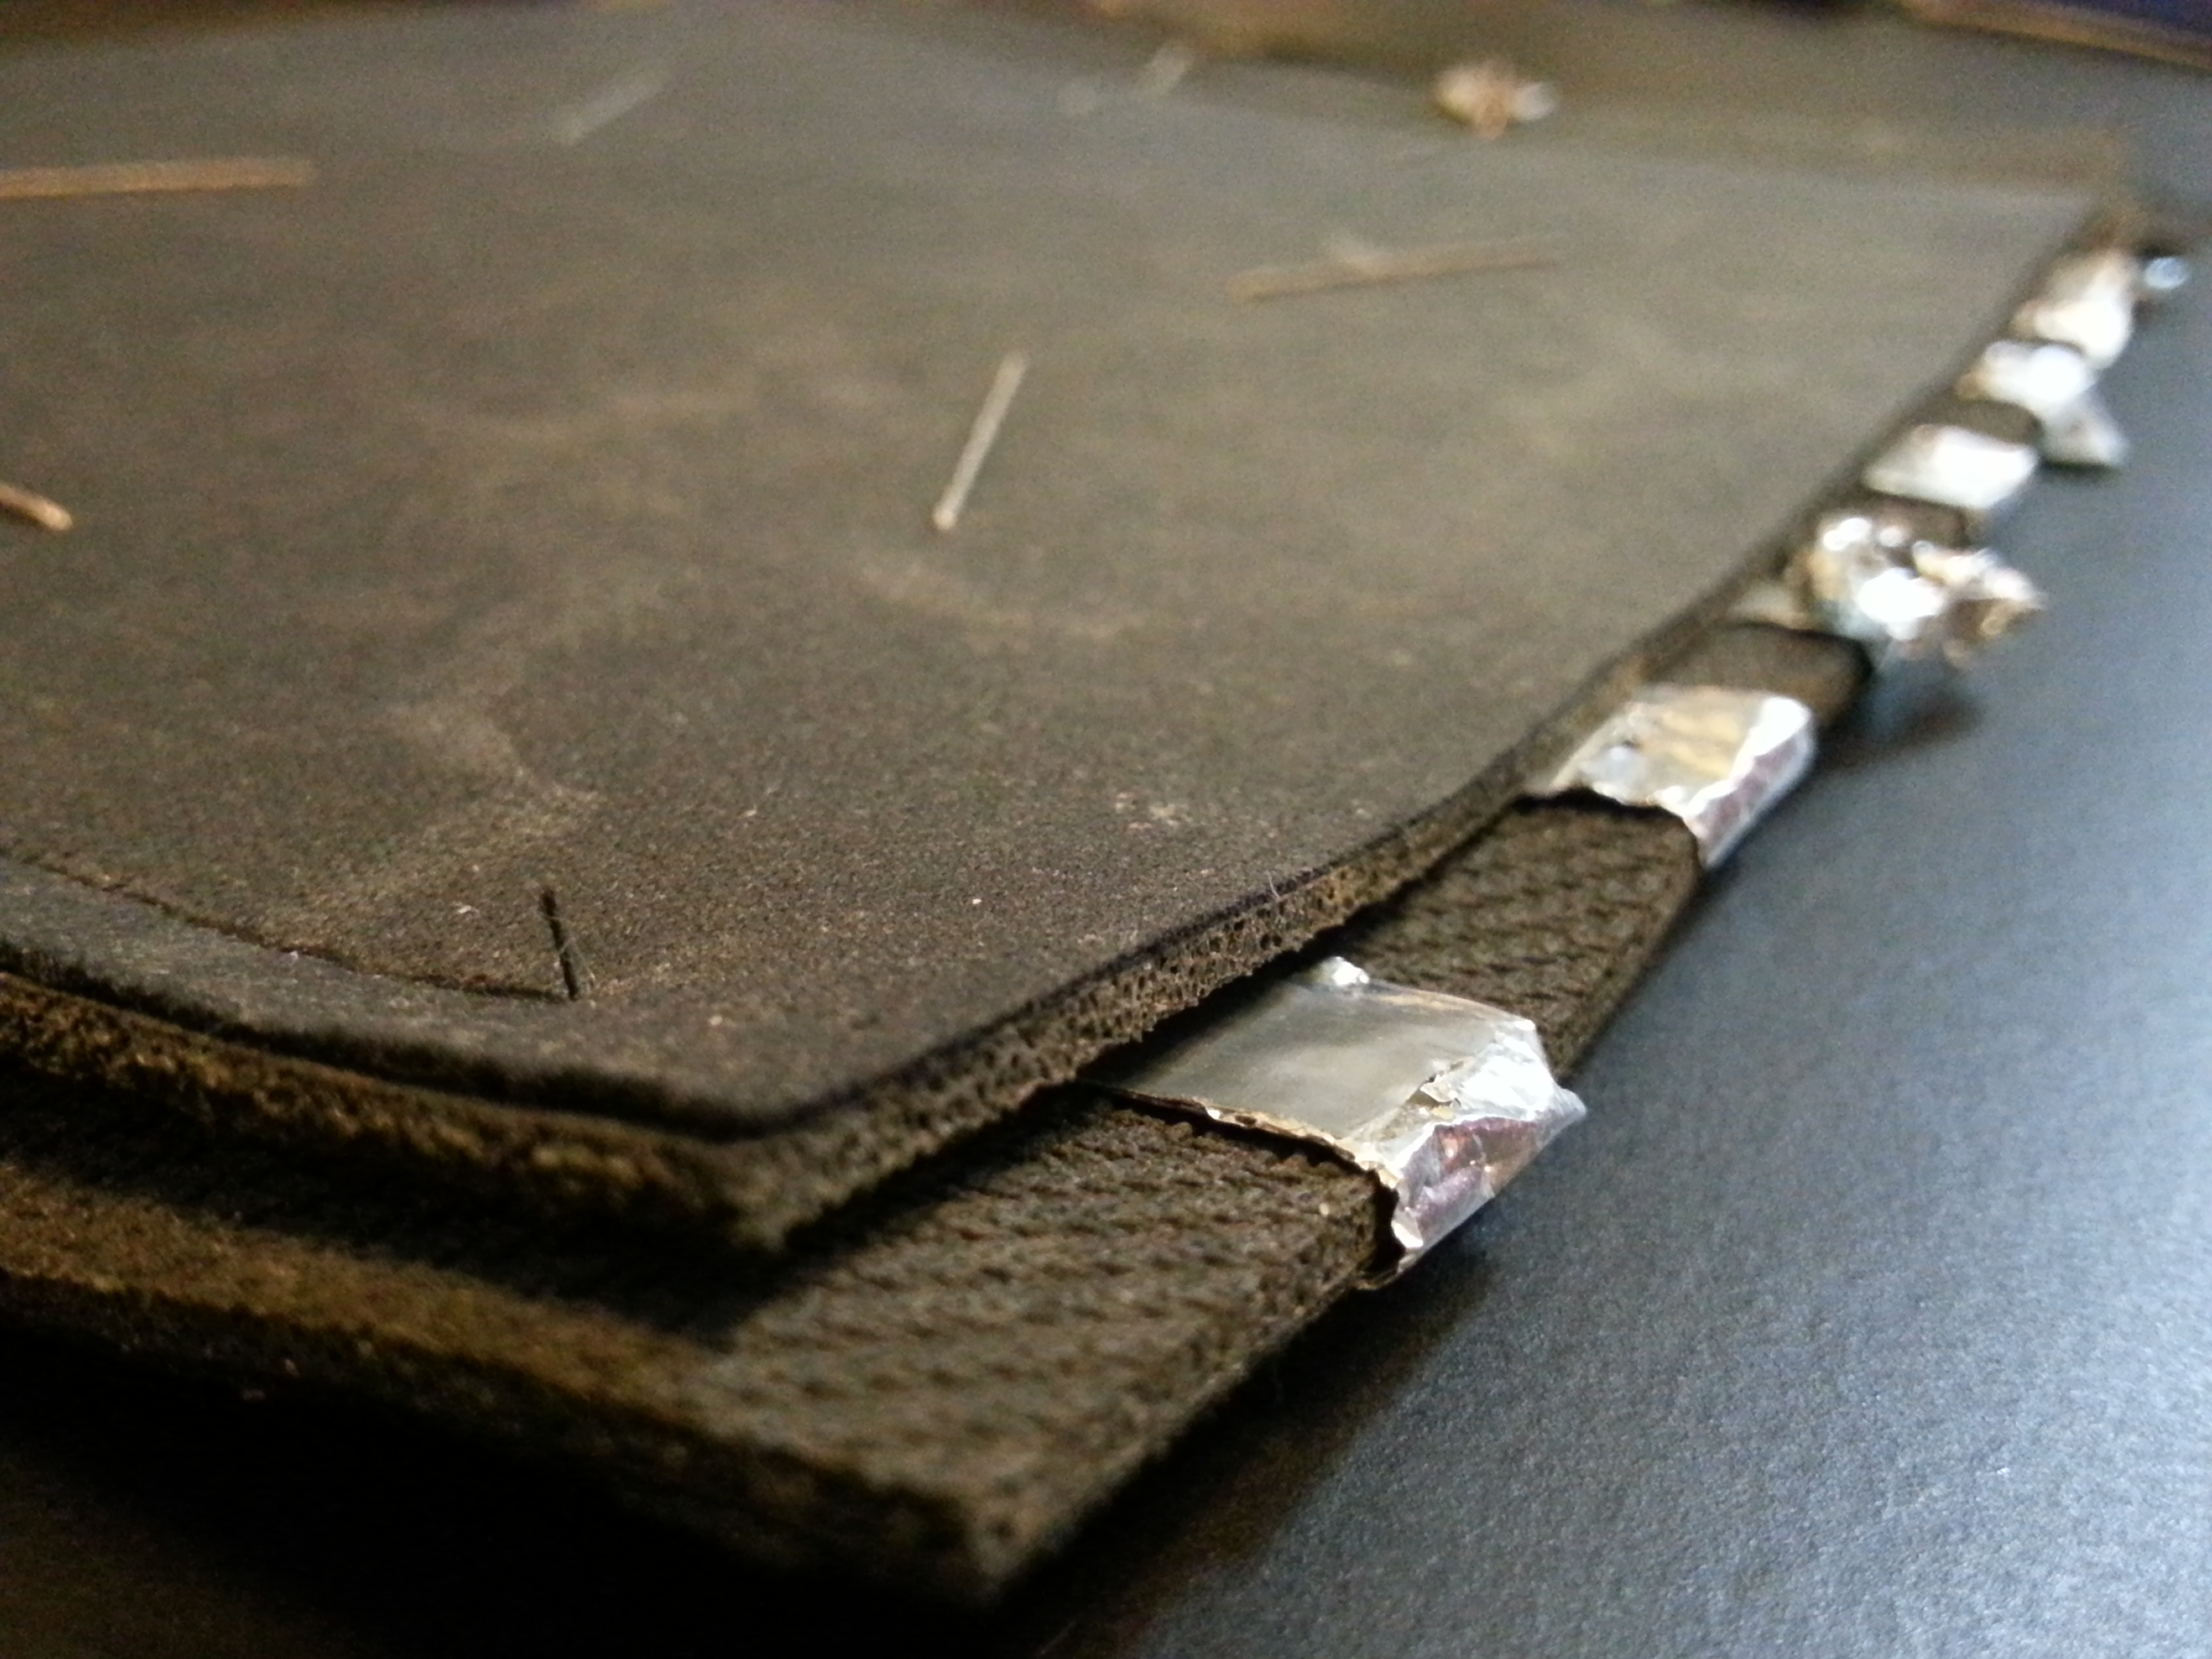
\includegraphics[width=.9\linewidth]{figures/touch/proto1_2}
  \caption{A close up of the materials}
\end{subfigure}
\caption{First iteration of our touch prototype}
\label{prototype_1}
\end{figure}

The top layer is made of 3 mm thick neoprene from an old mouse pad with one long conductive thread, made of stainless steel fibers, sewn into it.
Neoprene is easy to work with and gives a natural force-feedback when touched because of its thickness, \hl{but lacks the naturalness and flexibility of normal fabric used for clothing}.
The middle layer made from anti-static polymer bags that are normally used to protect electronics. 
Some types of anti-static bags, such as the ones we have used, acts as semi-conductors with piezoresistive capabilities and therefore fits in a FSR sensor.
We have tested three different types of anti-static bags, two semi transparent and one black, but only black ones, as seen in figure \todo{ref}, are piezoresistive.
We do not know if this is the general case as we only had a limited number of samples.
The bottom layer is another layer of neoprene, but with separate conductive stitchings for each of the 2x3 cells.

By sending 5v signal into the single top layer stitch, each of the six (2x3) bottom layer outputs can now be read on the Arduino after passing through the piezoresistive material.  
As pressure is applied to the different sections the voltage drop at the individual grid locations can now be measured with the analog input pins on the Arduino.
The ADC on the Arduino then translates the measured voltage, between 0-5v, into the amount of pressure that is applied to each of the cells, as a number between 0-1023.
The measured numbers will never reach the extremes as there is always some amount of resistance in the material.
A single layer of our anti-static bags have resistance values from around 180-200 KOhms, with little to no pressure applied, down to around 1.8 kOhms when pressed hard.
Depending on the piezoresistive material and the construction of the sensor, these values will vary, \citep{rosenberg2009unmousepad} reports values between 1.2 MOhms and 2.2 kOhms for their FSR ink.

Each of the cells acts, in principle, as a discrete sensor as they have their own individual output and are not influenced by each other

\begin{verbatim}
- Fokus paa konstruktionspricipper
- Inspireret af instructable
- 2x3 pad i neopren
- Hvert felt virker som en individuel tryksensor
- Meget simpel at prototype, viste os at princippet med conductive 
  thread og plast virker
- Simpel grafisk gui til test
- Ikke skalerbar, man kan ikke trykke uden for felterne og hvert felt
  bruger et input i audrino (2x3=6)
- Opdateringshastighed svarende til max baud-rate
\end{verbatim}
\subsection{Iteration 2}
\begin{verbatim}
- Fokus paa skalerbarhed
- Inspireret af rSkin
- 7x7 pad i sofastof
- Row/column tilgang reducerer antallet af arduino input til 7+7(additiv)
  i stedet for 7x7(multiplikativ),
  men kraever mere kompleks arduino kode, er derfor lang mere skalerbar end foer
- Reset knap til at kalibrere efter deformation
- Har samme oploesning som stoerrelsen (7x7), tryk imellem linjerne vil derfor blive 
  registeret som enten den ene eller anden linje
- Opdateringshastighed svarende til max baud-rate
\end{verbatim}
\subsection{Iteration 3}
See \ref{app:textile-touch} for schematics and \dots
\begin{verbatim}
- Fokus paa kode (gestures,resolution,performance)
- Inspireret af UnMousePad
- Samme fysiske prototype som iteration 2
- Interpolering muliggoere tryk mellem linjerne, 10x saa hoej oploesning dog udfald 
  og varierende praesision (vis vi har eksperimenteret med forskellige oploesninger)
- Forskellige visualiseringer til performance evaluering
- Integrering af gesture recognition og test miljoe til dette
- Haptisk feedback, vibration
- Udfordringer: praesision, performance 
  (max baud-rate for hurtigt til at java kunne foelge med)
\end{verbatim}